\begin{figure}[t]
    \centering
    \begin{subfigure}[b]{0.35\textwidth}
        \centering
        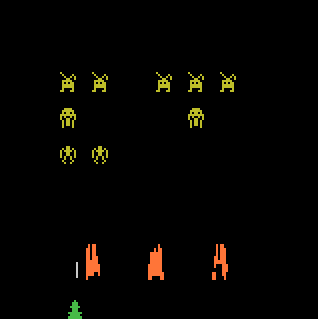
\includegraphics[width=\textwidth]
            {figures/explainability_reinforcement_learning/contrefactuel_1.png}
        \caption{}
        \label{fig:counterfactual_example_original}
    \end{subfigure}
    \hspace{0.02\textwidth}
    \begin{subfigure}[b]{0.35\textwidth}
        \centering
        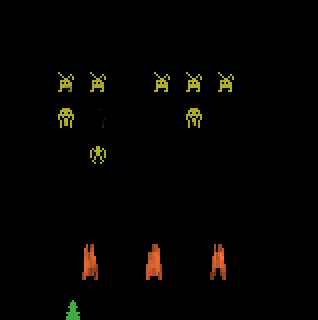
\includegraphics[width=\textwidth]
            {figures/explainability_reinforcement_learning/contrefactuel_2.png}
        \caption{}
        \label{fig:counterfactual_example_counterfactual}
    \end{subfigure}
    \caption{
        Counterfactual explanation of the agent's behavior for the Atari game \textit{Space Invaders} \cite{olson2021counterfactual}.
        Panel~\subref{fig:counterfactual_example_original} shows the original observation and panel~\subref{fig:counterfactual_example_counterfactual} the counterfactual observation produced by a generative model.
    }
    \label{fig:counterfactual_example}
\end{figure}
